\section{Opis działania i obsługi aplikacji}
    \subsection{Przewodnik}

        \subsubsection{Strona internetowa}
            Aplikacja znajduję się na zewnętrznym serwerze VPS i można ją przetestować bez uruchomiania lokalnie, dostępna jest pod adresem:
            \begin{itemize}
                \item \url{https://projekt.hu1.pl/}
            \end{itemize}

            \begin{figure}[!htb]
                \centering
                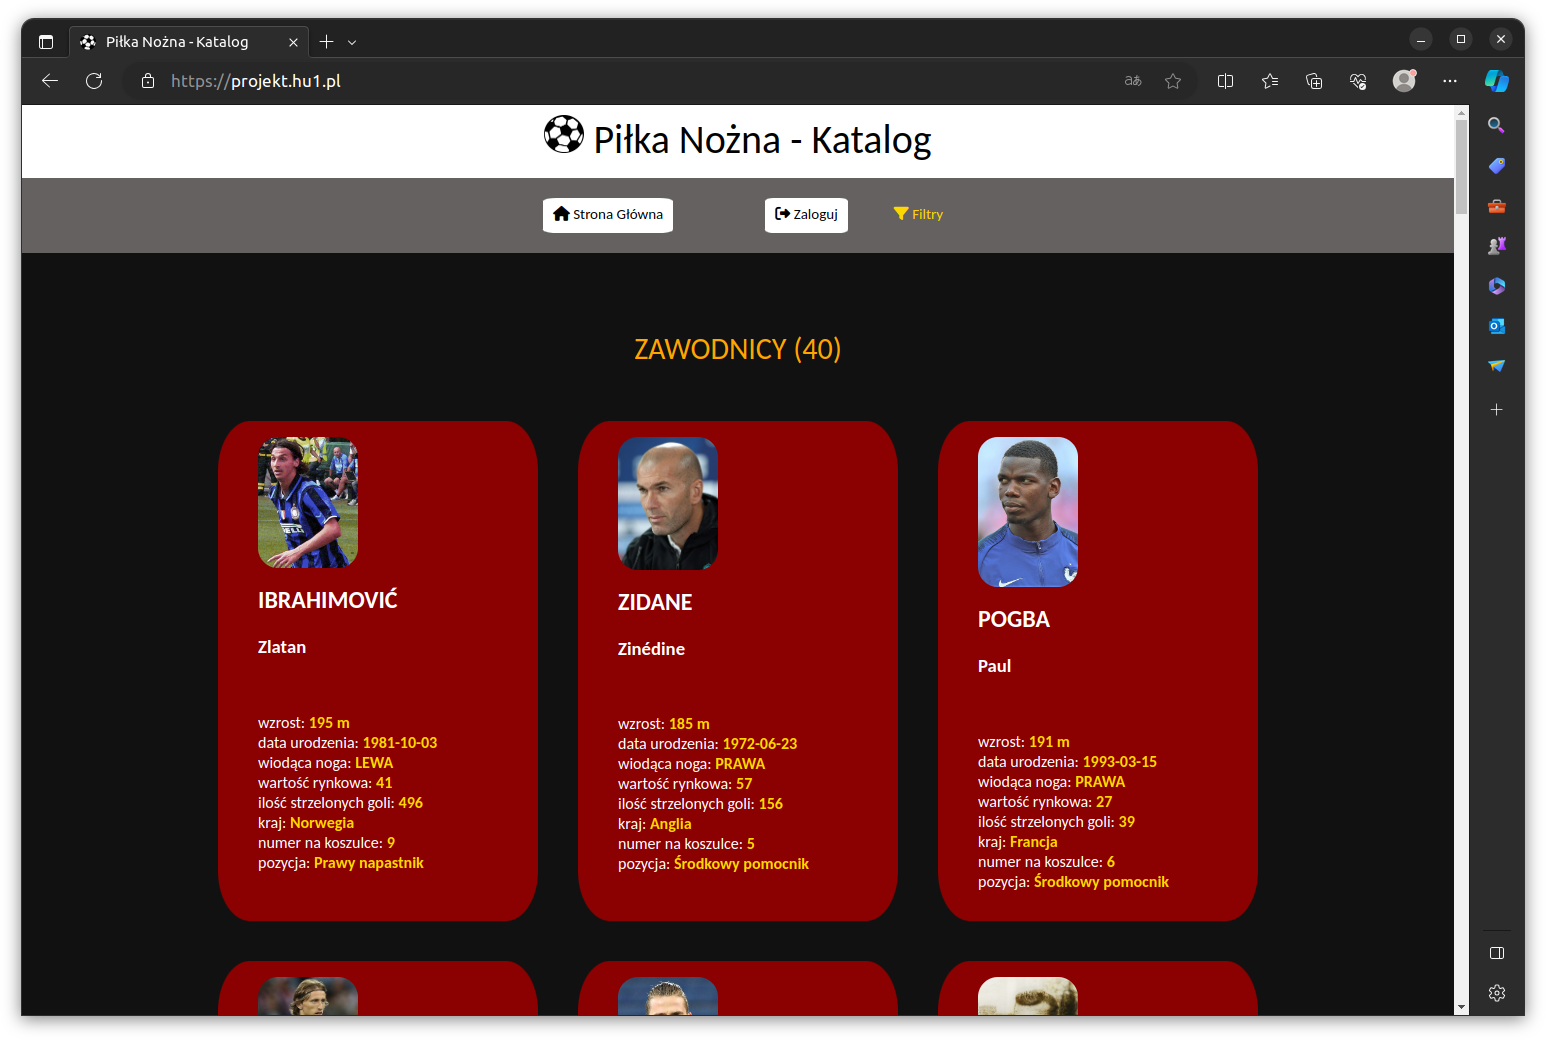
\includegraphics[width=0.6\textwidth]{przewodnik/home.png}
                \caption{Strona Główna}                
            \end{figure}

            \pagebreak

            \begin{figure}[!htb]
                \centering
                
\includegraphics[width=0.2\textwidth]{xiaomi}
                \caption{Strona Główna - wersja mobilna, Android}                
            \end{figure}
        \subsection{Wyświetlanie oraz filtrowanie piłkarzy}

        \begin{itemize}
            \item \url{https://projekt.hu1.pl/szukaj}
        \end{itemize}

            \begin{figure}[!htb]
                \centering
                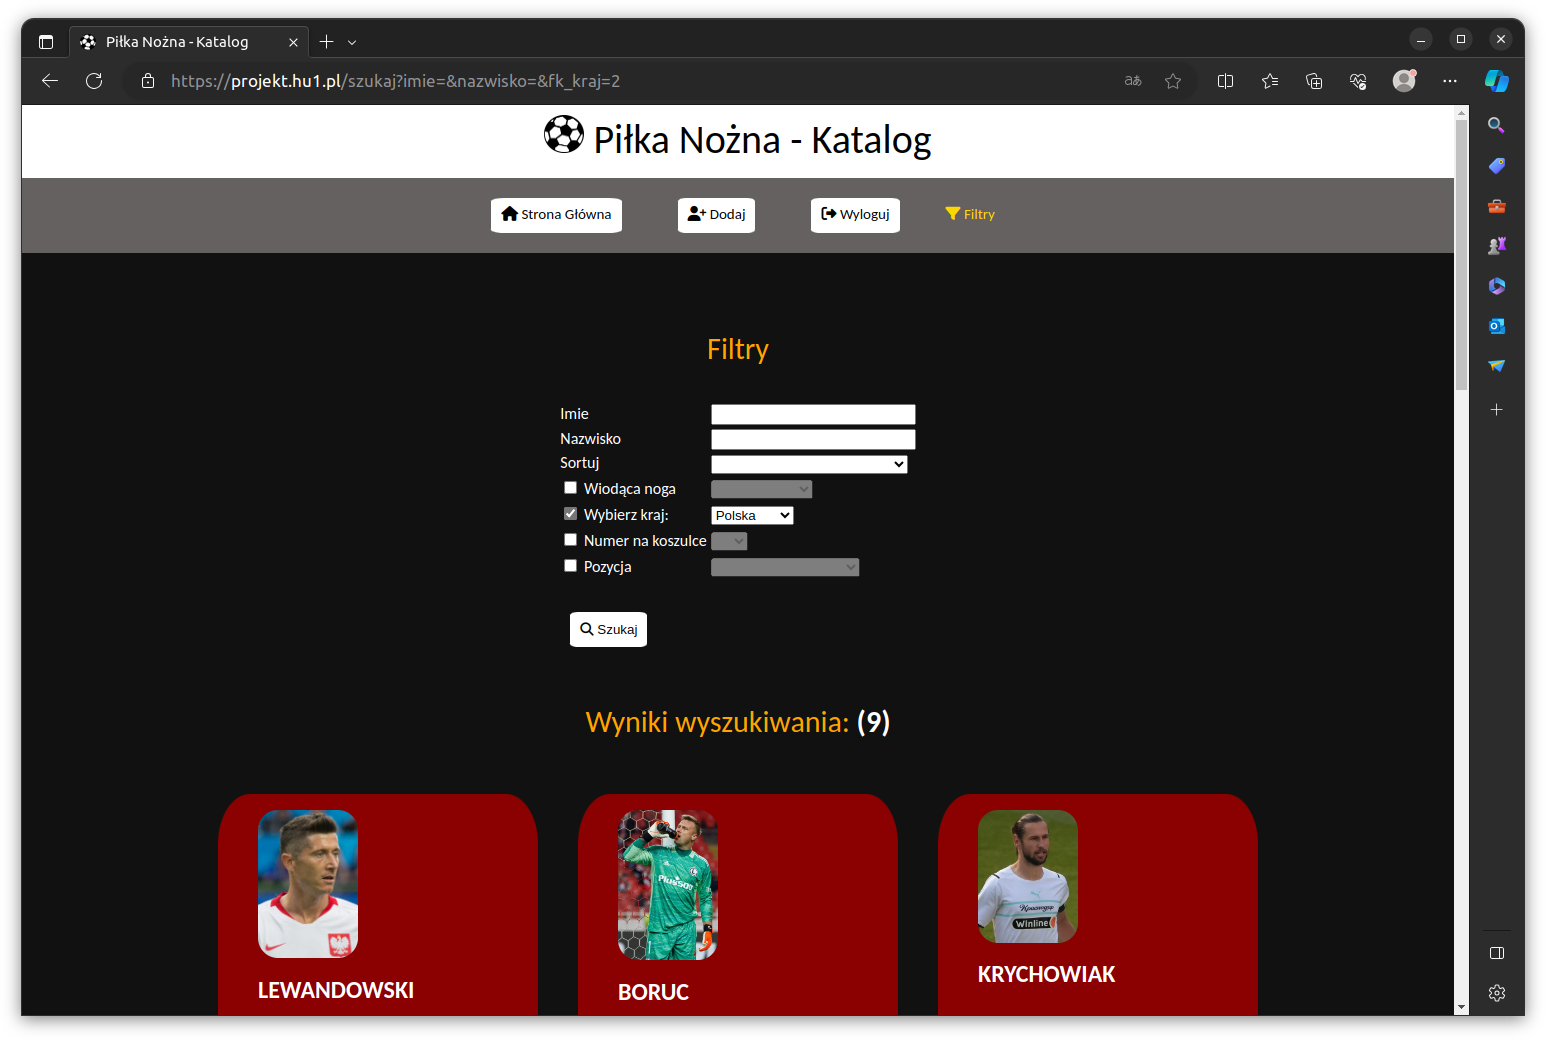
\includegraphics[width=0.6\textwidth]{przewodnik/filtry.png}
                \caption{Panel filtrowania}                
            \end{figure}
        
        \subsection{Panel Logowania}
            Panel logowania dostępny jest pod adresem:
            \begin{itemize}
                \item \url{https://projekt.hu1.pl/zaloguj}
            \end{itemize}

            Dane do logowania: 
            \begin{itemize}
                \item Użytkownik: \textbf{admin}
                \item Hasło: \textbf{admin}
            \end{itemize}

                \begin{figure}[!htb]
                    \centering
                    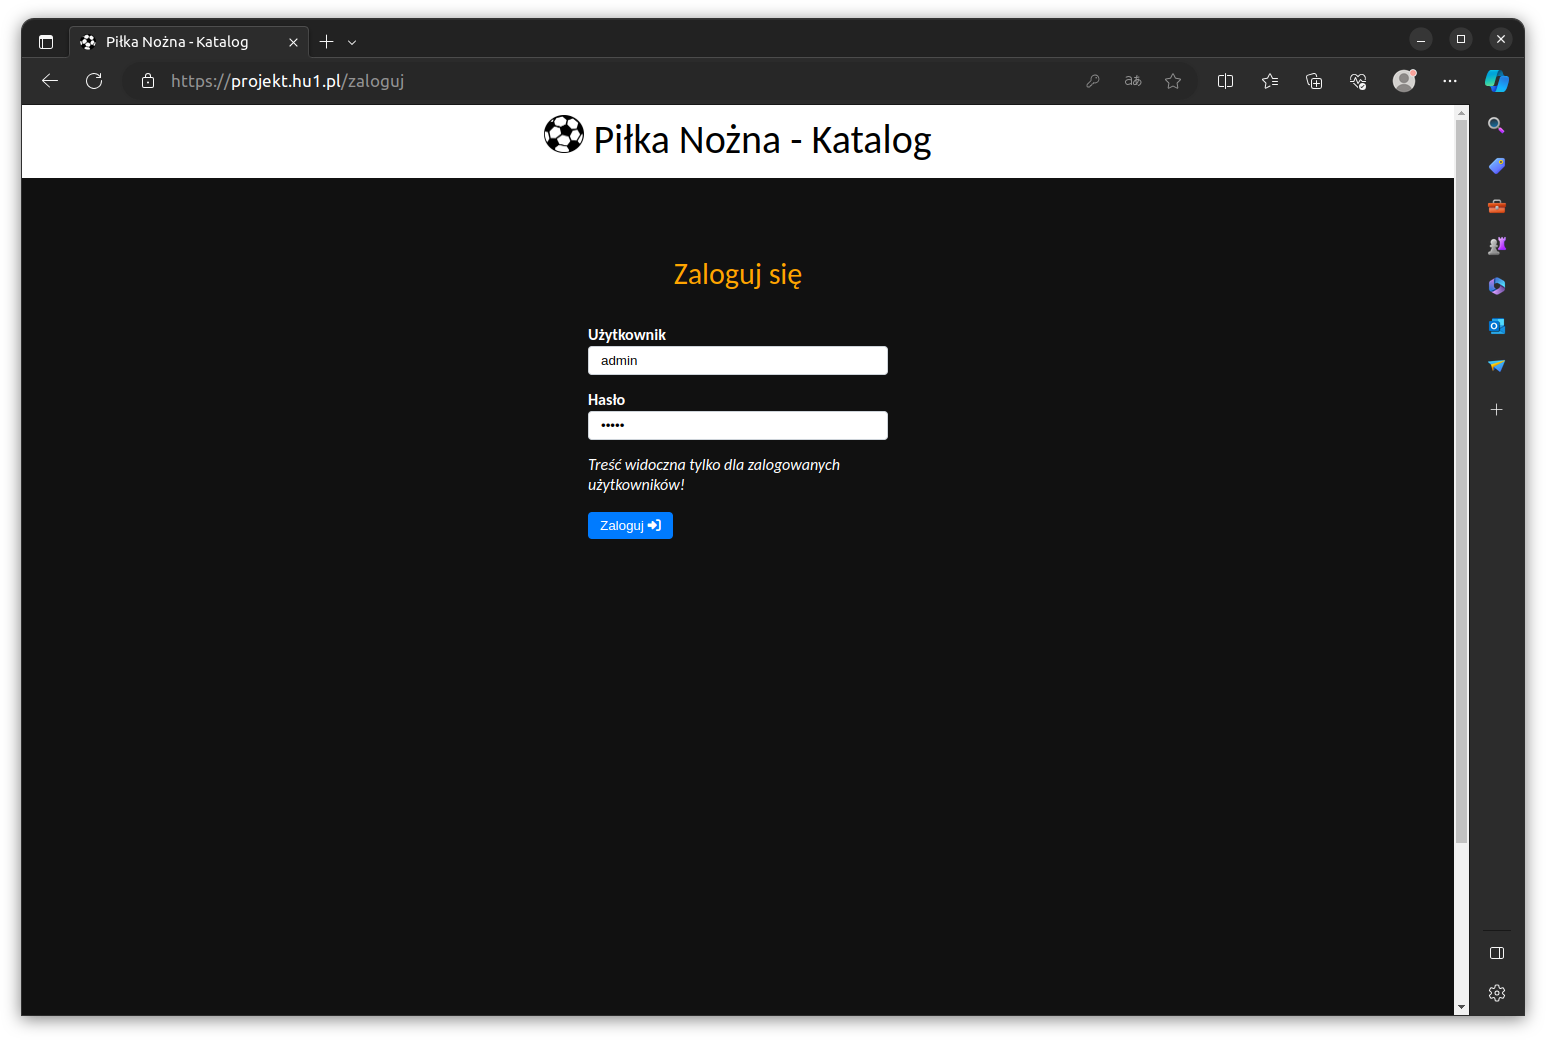
\includegraphics[width=0.6\textwidth]{przewodnik/login.png}
                    \caption{Panel logowania}                
                \end{figure}

        \pagebreak

        \subsection{Panel Administracyjny}
            Jako administrator użytkownik ma podniesione uprawienia i dodatkową zakładkę \textit{Dodaj} oraz przycisk \textit{Edytuj} lub \textit{Usuń} pod imieniem piłkarza.

            \begin{figure}[!htb]
                \centering
                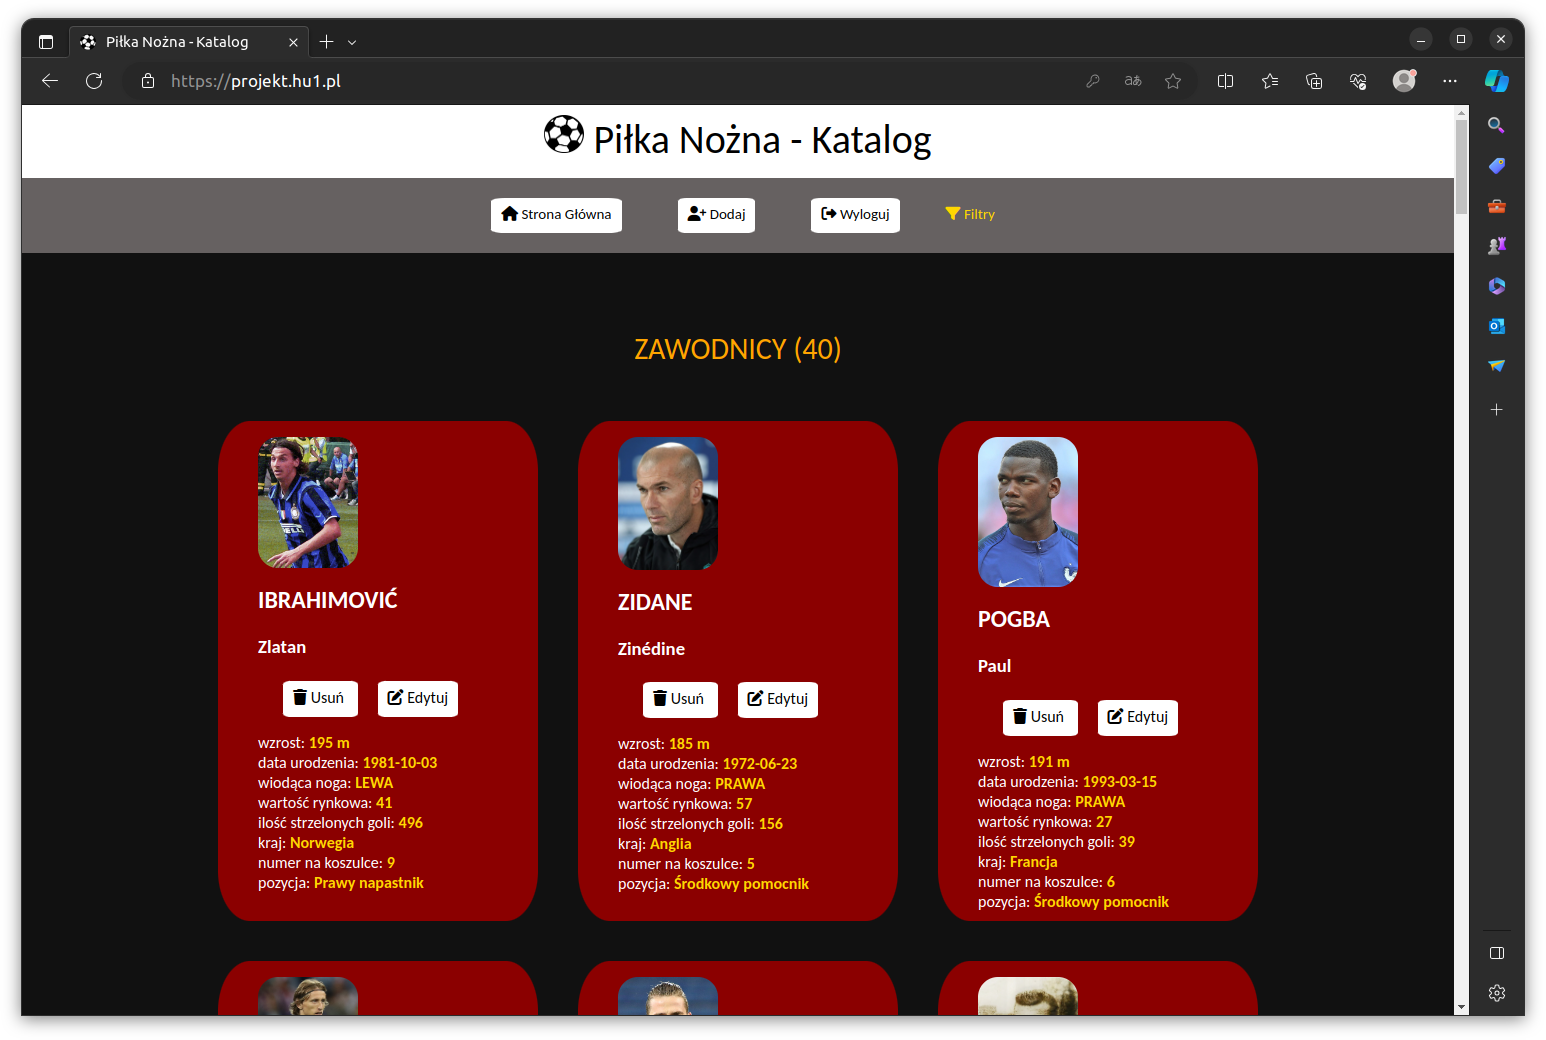
\includegraphics[width=0.6\textwidth]{przewodnik/admin.png}
                \caption{Panel Administracyjny}                
            \end{figure}

        \subsection{Modyfikowanie danych na temat piłkarzy}

        \subsubsection{Dodawanie piłkarza}

                \begin{itemize}
                    \item \url{https://projekt.hu1.pl/formularz_dodaj}
                \end{itemize}
                
        
                 Zdjęcie piłkarza jest pobierane z serwisu Wikipedia na podstawie \textbf{Imienia} oraz \textbf{Nazwiska}, o ile zawodnik posiada tam swój artykuł wraz ze zdjęciem - co zazwyczaj ma miejsce w 90\% przypadków. W sytuacji, gdy nie ma dostępnego zdjęcia piłkarza na stronie, automatycznie ustawiane jest domyślne zdjęcie anonimowego użytkownika.

                    \begin{figure}[!htb]
                        \centering
                        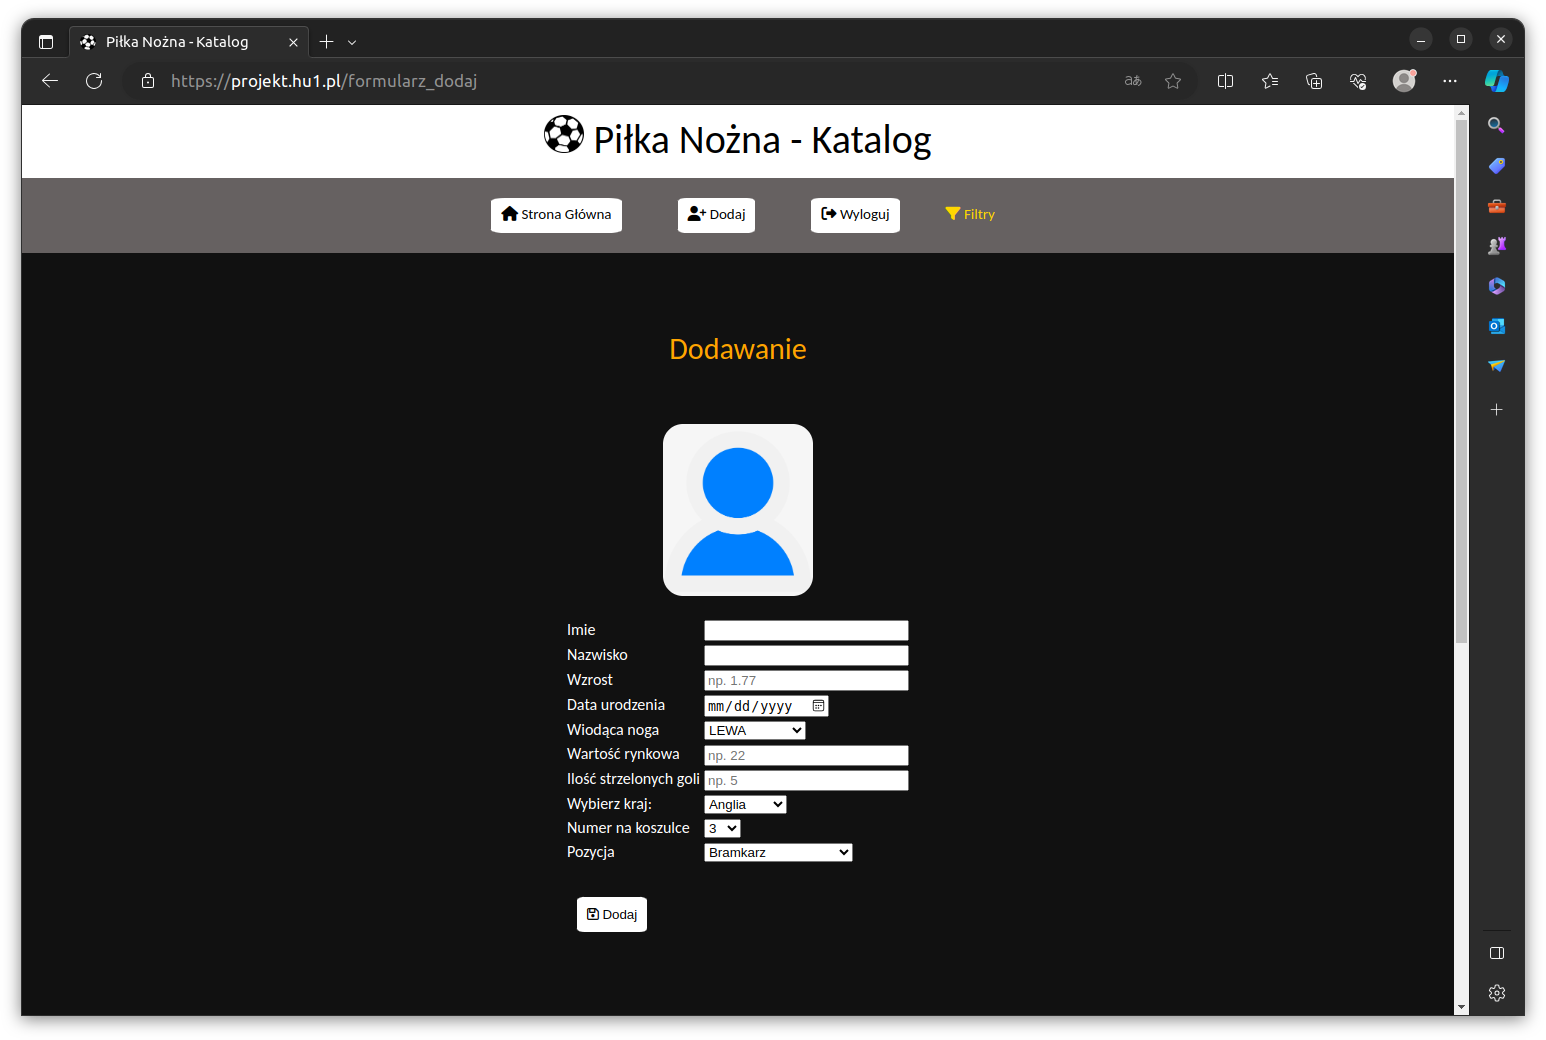
\includegraphics[width=0.6\textwidth]{przewodnik/dodaj.png}
                        \caption{Formularz, który umożliwia dodanie nowego Piłkarza}                
                    \end{figure}
                    \pagebreak

        \subsubsection{Usuwanie piłkarza}
        Przed usunięciem piłkarza pojawia się potwierdzenie. Można jeszcze anulować decyzję i zrezygnować z usunięcia lub potwierdzić.
            \begin{itemize}
                \item np. \url{https://projekt.hu1.pl/usun?id=79}
            \end{itemize}
            
            \begin{figure}[!htb]
                \centering
                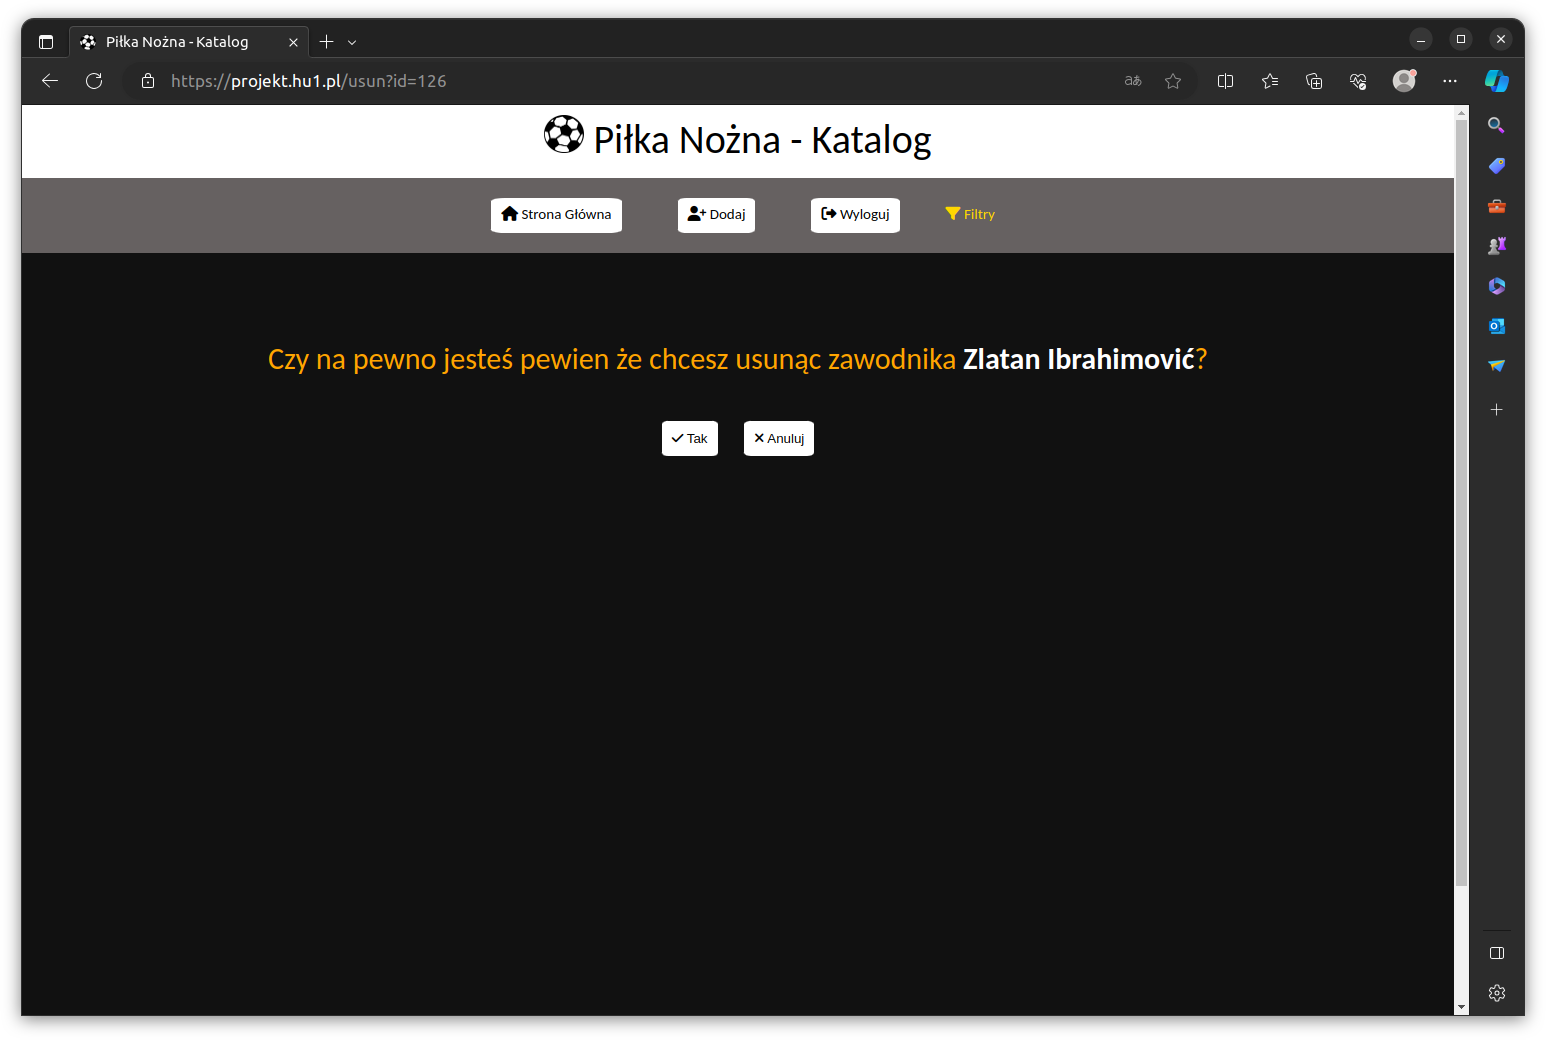
\includegraphics[width=0.6\textwidth]{przewodnik/usun.png}
                \caption{Potwierdzenie usunięcia Piłkarza}                
            \end{figure}
            \pagebreak

        \subsubsection{Edycja piłkarza}

            \begin{itemize}
                \item np. \url{https://projekt.hu1.pl/edytuj?id=79}
            \end{itemize}
            

            \begin{figure}[!htb]
                \centering
                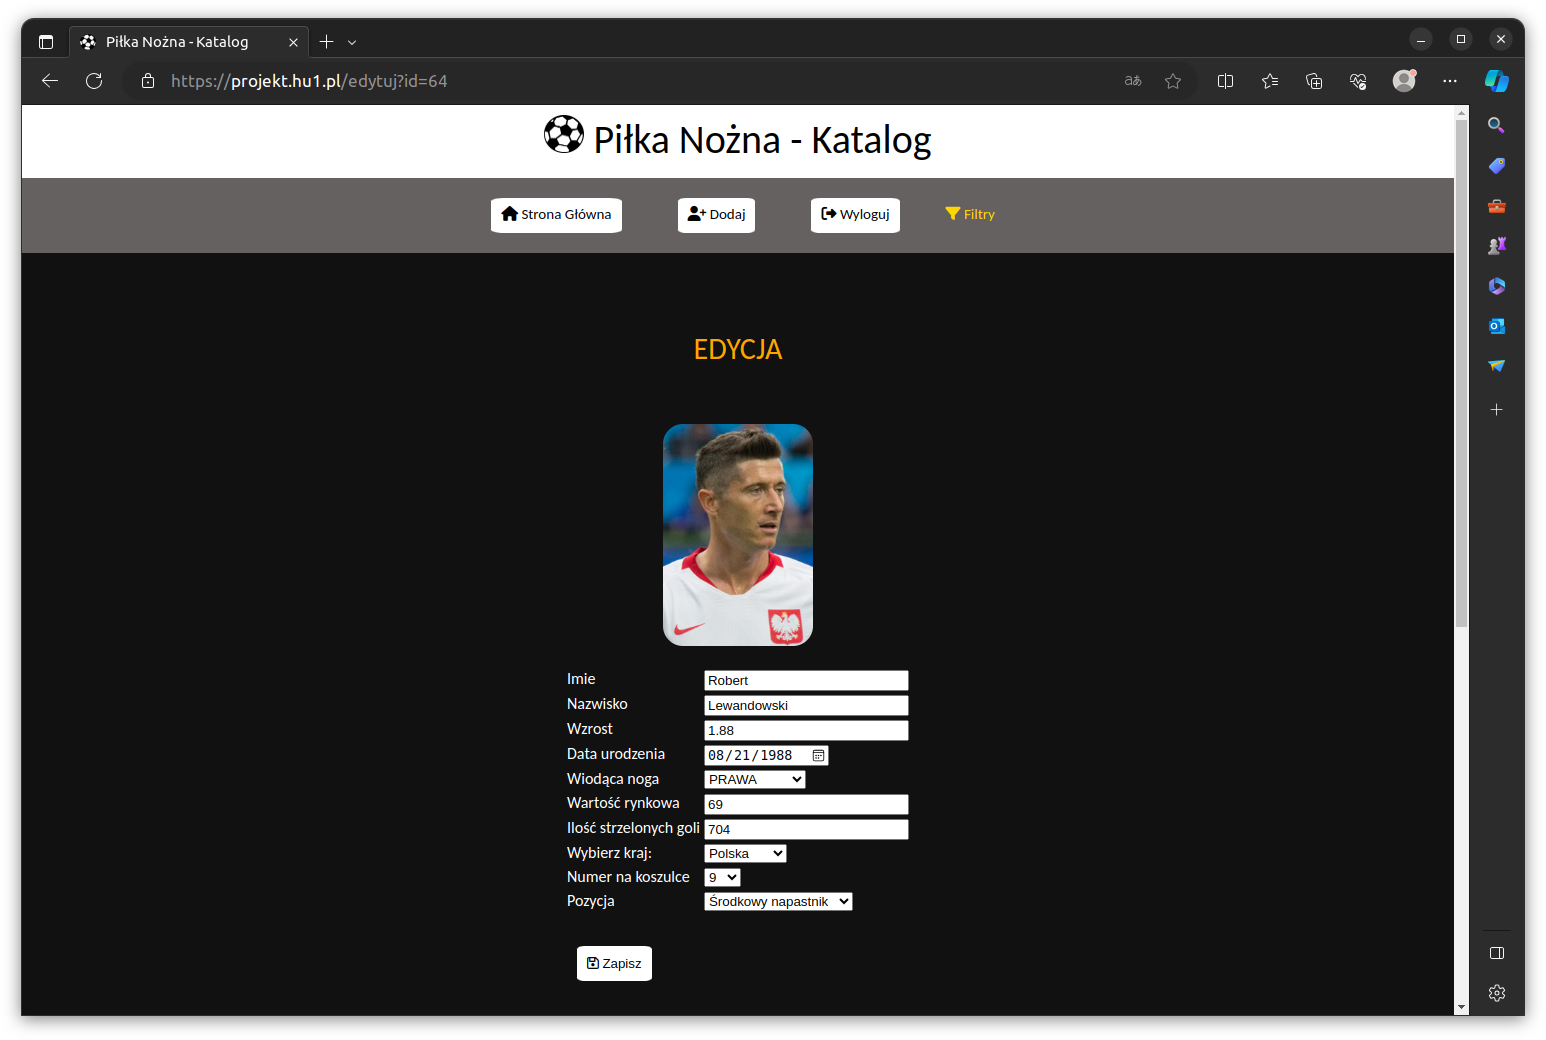
\includegraphics[width=0.6\textwidth]{przewodnik/edycja.png}
                \caption{Panel służący do edycji informacji na temat piłkarza}                
            \end{figure}